% ---------------------------------------------------------------------
% HEADER
% Formålet med å legge header til et eget dokument er å garantere at
% oppsettet av dokumentene er likt for alle løsningsforslagene.
% I headeren skjer følgende:
% (1) Dokumentet blir startet
% (2) Pakker blir importert
% ---------------------------------------------------------------------
% ---------------------------------------------------------------------
% HEADER
% Formålet med header er å importere de samme pakkene i alle dokumentene.
% ---------------------------------------------------------------------

% Sett opp dokumentet. Her kan 'twoside' brukes for printing
\documentclass[12pt, a4paper]{article}

% Vi trenger utf-8 for å bruke norske bokstaver: Æ, Ø, Å
\usepackage[utf8]{inputenc}

% Vi setter babel til norsk, da får dokumentegenskaper norske titler
\usepackage[norsk]{babel}

% For å kunne bruke grafikk
\usepackage{graphicx}
\newcommand{\figwidth}{0.75}

% Matematikkpakker fra AMS - American Mathematical Society
\usepackage{amsmath, amsthm, amsfonts, amssymb, mathtools}

% For eventuelle linker, e.g. \href{URL}{text}
\usepackage{hyperref}

% For headers og footers med eventuell logo
\usepackage{fancyhdr}

% Sett marginer manuelt
\usepackage[top = 3cm, left = 3cm, right = 3cm, bottom = 3cm]{geometry}

% For enkle lister, nyttig for oppgave a), b), c), ...
\usepackage[sharp]{easylist}

% Dersom flere kolonner er ønskelig i deler av dokumentet
\usepackage{multicol}

% For luft mellom paragrafer
\usepackage{parskip}

% For logikk assosiert med logoer
\usepackage{ifthen}

% For å finne totalt antall sider
\usepackage{lastpage}

% Annet
\usepackage{enumitem}

\usepackage{polynom}% Polynomer
\polyset{style=C, div=:}

\usepackage{systeme}% Likningssystemer

% Kan brukes når noe stryker ut noe, f.eks 1/n * n, her kan man ta \frac{1}{\cancel{n}} * \cancel{n}
\usepackage{cancel}



% ---------------------------------------------------------------------
% DOKUMENTVARIABLER
% ---------------------------------------------------------------------
\newcommand{\fagkode}{S2}
\newcommand{\semesteraar}{våren 2018}
\newcommand{\forfatter}{Tommy O.}
\newcommand{\dokumenttittel}{Løsningsforslag -- Eksamen \fagkode, \semesteraar}


% Set til 'true' og oppgi logo dersom du vil bruke en logo
\newboolean{bruklogo}
\setboolean{bruklogo}{true}
\newcommand{\logonavn}{figs/metis_akademiet_privatistskole_doclogo.png}

% ---------------------------------------------------------------------
% SETUP
% Formålet med å legge setup til et eget dokument å garantere at headers,
% footers, og øverste del av dokumentet er likt for alle
% løsningsforslagene.
% ---------------------------------------------------------------------
% ---------------------------------------------------------------------
% HEADER
% Formålet med setup er at dokumentene ser rimelig like ut.
% ---------------------------------------------------------------------


% ---------------------------------------------------------------------
% Alternativ font. Kommentert ut fordi Computer Modern (default) er pen
%\usepackage{kmath,kerkis}
%\usepackage[T1]{fontenc}
% ---------------------------------------------------------------------


% ---------------------------------------------------------------------
% Sett opp headers og footers
\ifthenelse{\boolean{bruklogo}}{
% Dersom logo skal brukes, sett logoen oppe til høyre med bredde 4 cm
	\rhead{\includegraphics[width=3.5cm]{\logonavn}}
}{
% Dersom logo ikke skal brukes, sett tom header
	\rhead{}
} 
\rfoot{\thepage}
\cfoot{}
\lhead{}
\lfoot{{\scriptsize Forbedringsforslag? Bidra på \url{https://github.com/tommyod/matte_eksamener_VGS}.}}
\renewcommand{\headrulewidth}{0pt}
% ---------------------------------------------------------------------


% ---------------------------------------------------------------------
% To streker under svaret
\def\answer#1{\underline{\underline{#1}}}
% ---------------------------------------------------------------------


% ---------------------------------------------------------------------
% Start selve dokumentet
% ---------------------------------------------------------------------

\begin{document}
\pagestyle{fancy}
{\bfseries \Large \dokumenttittel} \\
{ \footnotesize Laget av \forfatter 
	\hfill Sist oppdatert: \today 
	\hfill Antall sider: \pageref*{LastPage}}
\hrule
\vspace{1em}
\begin{center}
\fbox{\fbox{\parbox{.90\textwidth}{
	Dette dokumentet er open-source;
	alle kan bidra til å gjøre det bedre.
	Dersom du finner skrivefeil, matematiske feil, eller ser at forklaringene kan være bedre: ikke nøl med å sende inn en endring. 
	Du kan finne siste versjon, og bidra, på GitHub, se:
	\url{https://github.com/tommyod/matte_eksamener_VGS}
}}}
\end{center}


% ---------------------------------------------------------------------
% DOKUMENTSTART - Skriv løsningsforslaget nedenfor
% ---------------------------------------------------------------------	
\section*{Del 1 - uten hjelpemidler}
\subsection*{Oppgave 1}
\begin{easylist}[enumerate]
\ListProperties(Style2*=,Numbers=a,Numbers1=l,FinalMark={)})
# Vi skal derivere $f(x) = 2x^3 - 4x + 1$, og må bruke regelen $\left(x^n\right)' = nx^{n-1}$.
Vi får $f'(x) = 3\cdot2x^{3-1} - 4 x ^{1-1} + 0 = \answer{6x^2 - 4}$ som svar.

# Vi skal derivere $g(x) = x / e^x$. Det er fullt mulig å bruke brøkregelen for derivasjon, men man kan også skrive om funksjonen til produktet $g(x) = x e^{-x}$ og bruke produktregelen $(uv)' = u'v + uv'$.
Fordelen er at man slipper å huske brøkregelen.
Utregningen blir
\begin{align*}
	g'(x) =& \left(x \right)' e^{-x} + \left( e^{-x} \right)' x \\
	=& 1 e^{-x} + (-1)e^{-x}  x \\
	=& e^{-x} - e^{-x}  x \\
	=& \answer{e^{-x}(1 - x)}
\end{align*}
# Vi skal derivere $h(x) = \ln \left( x^2 + 4x\right)$, og må bruke kjernereglen $h'(x) = h'(u) \times u'(x)$, der $u$ er en kjerne.
Vi velger $u =x^2 + 4x$, da er $h(u) = \ln(u)$ og $h'(u) = 1/u$, slik at vi får
\begin{align*}
	h'(x) =& h'(u) \times u'(x) \\
	=& \left( \frac{1}{u}  \right) \times \left( 2x + 4 \right) \\
	=& \frac{2x + 4}{u} =  \answer{\frac{2x + 4}{x^2 + 4x}}
\end{align*}
\end{easylist}

\subsection*{Oppgave 2}
Vi skal løse likningssystemet nedenfor, og vi kan bruke to forskjellige metoder: innsetningsmetoden eller addisjonsmetoden.
Vi velger addisjonsmetoden.
\begin{align*}
	5 x + y + 2 z &= 0 \quad (\text{A})\\
	2 x + 3 y + z &= 3 \quad (\text{B})\\
	3 x + 2 y - z &= -3 \quad (\text{C})
\end{align*}
For å kvitte oss med variabelen $z$ regner vi ut to nye likninger $(\text{D}) = (\text{A}) - 2 \times (\text{B})$ og $(\text{E}) = (\text{A}) + 2 \times (\text{C})$ som følger.
\begin{align*}
	x - 5y  &= -6 \quad (\text{D})\\
	11 x + 5 y  &= -6 \quad (\text{E})
\end{align*}
Ved å legge disse sammen kvitter vi oss med $y$, får likningen $12x = -12$, og ser at $\answer{x = -1}$.
For å løse for $y$ setter vi $x=-1$ inn i likning $(\text{D})$ eller $(\text{E})$ og ser at $\answer{y = 1}$.
Nå vet vi verdiene til $x$ og $y$, og kan sette dette inn i $(\text{A})$, $(\text{B})$ eller $(\text{C})$ for å finne ut at $\answer{z = 2}$.
På eksamen bør du sette en prøve på svaret---det går fort og du vet umiddelbart om du har regnet riktig.

\subsection*{Oppgave 3}
I denne oppgaven ser vi på polynomet
\begin{equation*}
	P(x) = x^3 - 3x^2 - 13x + 15
\end{equation*}
\begin{easylist}[enumerate]
	\ListProperties(Style2*=,Numbers=a,Numbers1=l,FinalMark={)})
	# Generelt er et polynom $P(x)$ delelig på $(x-a)$ dersom $P(a) = 0$.
	Her er $P(x)$ delelig på $(x-1)$ ettersom 
	\begin{equation*}
	P(1) = (1)^3 - 3\cdot(1)^2 - 13\cdot(1) + 15 = 1 - 3 - 13 + 15 = \answer{0}.
	\end{equation*}
	# For å løse $P(x) > 0$ må vi først faktorisere $P(x)$.
	Vi vet at $(x-1)$ er en faktor, så vi utfører polynomdivisjonen \\
	\polylongdiv{x^3 - 3x^2 - 13x + 15}{x - 1} \\
	Vi kan bruke ABC-formelen eller en annen metode for å finne ut at $x^2 - 2x -15 = (x - 5)(x + 3)$. 
	Med andre ord er $P(x) = (x - 1)(x - 5)(x + 3)$, vi setter opp en fortegnslinje og kommer frem til at \answer{$P(X)> 0$ når $-3 < x < 1$ og når $x > 5$}.
\end{easylist}

\begin{center}
	
\includegraphics[width=0.8\linewidth]{figs/fortegn.pdf}
\end{center}

\subsection*{Oppgave 4}
\begin{easylist}[enumerate]
	\ListProperties(Style2*=,Numbers=a,Numbers1=l,FinalMark={)})
	# Vi bruker formelen $a_n = a_1 + d(n-1)$ og informasjonen fra oppgaven.
	\begin{equation*}
		a_n = a_1 + d(n-1) \quad \Rightarrow \quad 
%		a_4 = a_1 + d(3) \quad \Rightarrow \quad 
		a_4 = a_1 + 3d \quad \Rightarrow \quad 
		14 = 2 + 3d \quad \Rightarrow \quad
		d = 4
	\end{equation*}
	Nå vet vi at differansen $d=4$ i den artimetiske rekken, vi setter inn og får
	\begin{equation*}
		a_n = a_1 + d(n-1) \quad \Rightarrow \quad  
		a_n = 2 + 4(n-1) \quad \Rightarrow \quad
		\answer{a_n = 4n - 2}.
	\end{equation*}
	# Vi bruker summeformelen for en aritmetisk rekke til å regne ut summen for en generell $n$, og løser deretter når $n = 100$.
	For en generell $n$ har vi at
	\begin{equation*}
		S_n = \left(\frac{a_1 + a_n}{2}\right) n 
		= \left(\frac{2 + 4n - 2}{2}\right) n
		= \left( 2n\right) n = 2n^2.
	\end{equation*}
	Når $n= 100$, blir $S_n = S_{100} = 2 \cdot (100)^2 = \answer{20000}$.
\end{easylist}

\subsection*{Oppgave 5}
\begin{easylist}[enumerate]
	\ListProperties(Style2*=,Numbers=a,Numbers1=l,FinalMark={)})
	# En geometrisk rekke $a_1(1 + k + k^2 + k^3 + \dots)$ konvergerer dersom $-1 < k < 1$.
	Her er $a_1 = 3$, $a_2 = 3/4$ og $a_3 = 3/16$, og $k = 1/4$ fordi hvert ledd er lik $1/4$ ganget med det foregående leddet.
	\answer{Rekken konvergerer fordi $k = 1/4$.}
	Summen av den uendelige geometriske rekken regner vi ut som
	\begin{equation*}
		S_{\infty} = a_1 \left(\frac{1}{1 - k}\right) 
		= 3 \left(\frac{1}{1 - \frac{1}{4}}\right) 
		= 3 \left(\frac{1}{\frac{3}{4}}\right)
		=  3 \left(\frac{4}{3}\right)
		=  \answer{4}
	\end{equation*}
	# Desimaltallet $0.242424\dots$ kan skrives som 
	$\frac{24}{100} + \frac{24}{100^2} + \frac{24}{100^3} + \dots$
	fordi desimalene 24 gjentar seg, og å dele på $100$ flytter desimalene to plasser til høyre. 
	Første ledd blir $0.42$, andre ledd blir $0.0042$, tredje ledd blir $0.000042$ og så videre---da blir summen $0.424242\dots$.
	For å skrive $0.242424\dots$ som en brøk bruker vi formelen for sum av en uendelig geometrisk rekke. 
	Vi vet at
	\begin{equation*}
		a_1 (1 + k + k^2 + \dots) = a_1 \left(\frac{1}{1 - k}\right),
	\end{equation*}
	og ved å trekke fra $a_1$ på begge sider ser vi at
	\begin{equation*}
		a_1 (k + k^2 + \dots) = a_1 \left(\frac{1}{1 - k} - 1\right).
	\end{equation*}
	Venstresiden likner nå på summen. 
	Vi setter inn $a_1 = 24$ og $k = 1/100$ og får
	\begin{equation*}
		a_1 \left(\frac{1}{1 - k} - 1\right) =
		24 \left(\frac{1}{1 - \frac{1}{100}} - 1\right) = 
		24 \left(\frac{1}{\frac{99}{100}} - 1\right) = 
		24 \left(\frac{100}{99} - \frac{99}{99}\right) = \answer{\frac{24}{99}}
	\end{equation*}
\end{easylist}

\subsection*{Oppgave 6}
I denne oppgaven ser vi på funksjonen
\begin{equation*}
	f(x) = \frac{6}{1 + e^{-x}} = 6 \left( 1 + e^{-x} \right)^{-1}.
\end{equation*}
\begin{easylist}[enumerate]
	\ListProperties(Style2*=,Numbers=a,Numbers1=l,FinalMark={)})
	# Grafen til $f(x)$ er alltid stigende dersom den deriverte er positiv for alle verdier av $x$.
	Vi deriverer funksjonen ved hjelp av kjerneregelen. Vi velger $u = 1 + e^{-x}$ som kjerne, da er $f(u) = 6u^{-1}$, og vi får at
	\begin{align*}
		f'(x) =& f'(u) \times u'(x) \\
		=& 6(-1)u^{-2} \times \left((-1) e^{-x}\right) \\
		=& \frac{6e^{-x}}{u^2} = \frac{6e^{-x}}{\left(1 + e^{-x}\right)^2}
	\end{align*}
	La os nå undersøke $f'(x)$.
	Telleren er alltid positiv fordi $e^{-x}$ alltid er positiv, nevneren er alltid positiv fordi $(1 + e^{-1})$ alltid er større enn 1, og å ta et tall som er større enn 1 i andre gir alltid i et positivt resultat.
	Både telleren og nevneren er positive for alle $x$, og da må $f'(x)$ alltid være positiv, og da stiger $f(x)$ alltid.

	# Vi ser på nevneren $(1 + e^{-x})$.
	Funksjonen $e^{-x}$ er alltid positiv, så da vet vi at
	\begin{equation*}
		1 < 1 + e^{-x} < \infty.
	\end{equation*}
	Når $1 + e^{-x}$ blir stor, går $f(x)$ mot $0$.
	Når $1 + e^{-x}$ går mot $1$, går $f(x)$ mot $6$.
	Da vet vi at $\answer{0 < f(x) < 6}$ for alle verdien av $x$.
	# En funksjon har ventepunkt når den dobbelderiverte skifter fortegn.
	Vi regner ut den dobbelderiverte fra $f'(x) = \frac{6e^{-x}}{\left(1 + e^{-x}\right)^2} = 6e^{-x} \left(1 + e^{-x}\right)^{-2} $ ved hjelp av produktregelen og kjerneregelen slik
	\begin{align*}
		f''(x) &= \left[ 6e^{-x} \right]' \left(1 + e^{-x}\right)^{-2} + 6e^{-x} \left[ \left(1 + e^{-x}\right)^{-2} \right]' \\
		&=  -6e^{-x}  \left(1 + e^{-x}\right)^{-2} + 6e^{-x} (-2)  \left(1 + e^{-x}\right)^{-3} (-1) e^{-x}  \\
		&=  \frac{-6e^{-x}}{\left(1 + e^{-x}\right)^{2}}  + \frac{12\left(e^{-x}\right)^2}{\left(1 + e^{-x}\right)^{3}} =
		 \frac{-6e^{-x} \left(1 + e^{-x}\right)}{\left(1 + e^{-x}\right)^{3}} 
		  + \frac{12\left(e^{-x}\right)^2}{\left(1 + e^{-x}\right)^{3}}\\
		 &=  \frac{-6e^{-x} \left(1 + e^{-x}\right) + 12\left(e^{-x}\right)^2}{\left(1 + e^{-x}\right)^{3}}
	\end{align*}
	Nevnerer er alltid positiv, så vi undersøker når telleren er lik null.
	Vi ser at
	\begin{equation*}
		-6e^{-x} \left(1 + e^{-x}\right) + 12\left(e^{-x}\right)^2 = 
		-6e^{-x} - 6\left(e^{-x}\right)^2 + 12\left(e^{-x}\right)^2 = 
		e^{-x} \left(-6 + 6 e^{-x}\right).
	\end{equation*}
	Med andre ord er $f''(x) = 0$ når $\left(-6 + 6 e^{-x}\right) = 0$,
	og dette skjer når $x = 0$, da bytter også $f''(x)$ fortegn og vi har et vendepunkt.
	For å finne $y$-verdien regner vi ut at $y = f(0) = 6 / (1 + e^{-0}) = 3$,
	da er \answer{$(0, 3)$ et vendepunkt}.
	# TODO: SKISSE HER.
\end{easylist}

\subsection*{Oppgave 7}
\begin{easylist}[enumerate]
	\ListProperties(Style2*=,Numbers=a,Numbers1=l,FinalMark={)})
	# Den stokastiske variabelen $X$ er binomisk fordelt med $p = \text{gunstige} / \text{mulige} =  6/10 = 0.6$ og $n = 10$ fordi å trekke kuler med tilbakelegging er en serie uavhengige deleksperimenter med konstant sannsynlighet $p$.
	# Gitt $p = 6/10 = 0.6$ og $n = 10$ regner vi slik
	\begin{align*}
		\operatorname{E}(X) &= np = 10 \left(\frac{6}{10}\right) = \answer{6} \\
		\operatorname{Var}(X) &= np(1-p) = 10 \left(\frac{6}{10}\right) \frac{4}{10} = \frac{24}{10} = \answer{2.4} 
	\end{align*}
\end{easylist}

\subsection*{Oppgave 8}
\begin{easylist}[enumerate]
	\ListProperties(Style2*=,Numbers=a,Numbers1=l,FinalMark={)})
	# La $X$ være vekten til et rugbrød.
	Da er $X$ normalfordelt med forventningsverdi $\mu = 1.00$ og standardavvik $\sigma = 0.05$.
	For å regne ut $P(0.9 < X < 1.1)$ må vi først gjøre om slik at vi får to ``mindre enn'' sannsynligheter (fordi det er dette som finnes i tabellen), og deretter standardisere ved formelen $Z = (X - \mu) / \sigma$.
	Vi regner slik
	\begin{align*}
		P(0.9 < X < 1.1) &= P(X < 1.1) - P(X < 0.90) \\
		&= P\left( \frac{X - \mu}{\sigma} <  \frac{1.1 - 1}{0.05} \right) -
		P\left( \frac{X - \mu}{\sigma} <  \frac{0.9 - 1}{0.05} \right) \\
		&= P\left( Z <  \frac{0.1}{0.05} \right) -
		P\left( Z <  \frac{-0.1}{0.05} \right) \\
		&= P\left( Z <  2 \right) -
		P\left( Z <  -2 \right) \\
		&= 0.9772 - 0.0228 \qquad (\text{fra tabell}) \\
		&= \answer{0.9544 = 95.4 \%}
	\end{align*}
	# La $S = X_1 + X_2 + \dots + X_{100}$ være summen av 100 rugbrød.
	Når alle $X$'ene er normalfordelte vil summen være normalfordelt.
	Selv om $X$'ene ikke hadde vært normalfordelte, ville summen vært tilnærmet normalfordelt på grunn av sentralgrenseteoremet.
	For en sum av stokastiske variabler regner vi forventningen $\mu_S$ og standardavviket $\sigma_S$ til summen $S$ slik
	\begin{align*}
		\operatorname{E}(S) &= \mu_S = n \mu = 100 \cdot 1 = 100 \\
		\operatorname{SD}(S) &= \sigma_S = \sqrt{n} \sigma = \sqrt{100} \cdot 0.05 = 0.5 \\
	\end{align*}
	Når regner vi ut på samme måte som i forrige deloppgave.
	\begin{align*}
		P(99.5 < S < 100.5) &= P(X < 100.5) - P(X < 99.5) \\
		&= P\left( \frac{S - \mu}{\sigma} <  \frac{100.5 - 100}{0.5} \right) -
		P\left( \frac{S - \mu}{\sigma} <  \frac{99.5 - 100}{0.5} \right) \\
		&= P\left( Z <  1 \right) -
		P\left( Z <  -1 \right) \\
		&= 0.8413 - 0.1587 \qquad (\text{fra tabell}) \\
		&= \answer{0.6826 = 68.3 \%}
	\end{align*}
\end{easylist}

\subsection*{Oppgave 9}
La oss først se på noen generelle egenskaper til funksjonen $g(x) = a f(x) + b$ før vi setter inn $a=-5$ og $b=3$ og løser oppgaven.
Den deriverte til $g(x)$ er gitt ved
\begin{equation*}
	g'(x) = \left[ a f(x) + b \right]' = a f'(x),
\end{equation*}
og da er $g'(x) = 0$ når $f'(x) = 0$, og motsatt.
Med andre ord har bunn- og toppunktene til $g(x)$ og $f(x)$ de samme $x$-verdiene. Dette gir mening, fordi å plusse på $b$ flytter grafen opp langs $y$-aksen, mens å gange med $a$ skalerer grafen---ingen av regneoperasjonene flytter grafen langs $x$-aksen.\footnote{Transformasjonen som flytter en funksjon er $g(x) = f(x - a)$, som flytter $f$ med $a$ mot høyre.}
Vi må derimot passe oss for $a < 0$; dersom $a$ er negativ snur grafen seg om $x$-aksen slik at toppunkter blir til bunnpunkter og motsatt.

La oss gå bort fra generell teori og løse oppgaven. \\
I toppunktet $(2, 3)$ er $f'(x) = 0$, da er $g'(x) = -5 f'(x) = -5 \times 0 = 0$, så $g(x)$ har et bunnpunkt når $x = 2$. 
Legg merke til at multiplikasjon med $-5$ gjør toppunkt til bunnpunkt og motsatt. 
I punktet $x=2$ er $y = g(2) = -5 f(2) + 3 = -5 \cdot 3 +3 = -12$. 
Da vet vi at \answer{$(2, -12)$ er et bunnpunkt} til $g(x)$.

I bunnpunktet $(3, -4)$ er $f'(x) = 0$, da er $g'(x) = -5 f'(x) = -5 \times 0 = 0$, så $g(x)$ har et toppunkt når $x = 3$. 
Videre er $y = g(3) = -5 f(3) + 3 = -5 \cdot (-4) + 3 = 23$. 
Da har vi at \answer{$(3, 23)$ er et toppunkt} til $g(x)$.









\section*{Del 2 - med hjelpemidler}

\subsection*{Oppgave 1}
\begin{easylist}[enumerate]
	\ListProperties(Style2*=,Numbers=a,Numbers1=l,FinalMark={)})
	# Vi legger punktene for $K(x)$ inn i Geogebra, velger ``Regresjonsanalyse'' og undersøker et tredjegradspolynom, som vist i Figur \ref{fig:del2_oppg1a}.
	Vi får forslaget $K(x) = 0.05x^3 - 1.97x^2 + 39.42x + 501.02$.
	Inntekten er $I(x) = 80x$ fra oppgaveteksten, da blir overskuddet
	\begin{align*}
		O(x) &= I(x) - K(x) \\
		&= 80x -\left[ 0.05x^3 - 1.97x^2 + 39.42x + 501.02 \right] \\
		&= - 0.05x^3 + 1.97x^2 + 40.58x - 501.02
	\end{align*}
	Dette stemmer godt overens med $O(x)$ som gitt i oppgaveteksten.
	\begin{figure}[ht!]
		\centering
		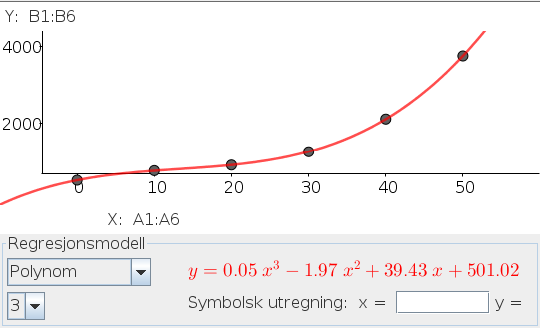
\includegraphics[width=0.7\linewidth]{figs/del2_oppg1a}
		\caption{Løsning på oppgave 1 a, del 2. Koeffisientene passer godt med $O(x)$.}
		\label{fig:del2_oppg1a}
	\end{figure}
	# Se Figur \ref{fig:del2_oppg1bc} for et plott av $O(x)$.
	
	# Ettersom $O(x) = I(x) - K(x)$, er $I'(x) = K'(x)$ når $O'(x) = 0$.
	Da har vi et ekstremalpunkt, vi finner dette med Geogebra-kommandoen\\
	\verb|Ekstremalpunkt(O, 0, 60)|. \\
	Punktet er $(34.57, 1240.84)$.
	Verdien av $x$ som maksimerer $O(x)$ er den vinningsoptimale produksjonsmengden, det vil si produksjonsmengden som gir størst overskudd.
	Ettersom $O(34) = 1239.8$ og $O(35)=1240.25$, er den \answer{vinningsoptimale produksjonsmengden lik $x = 35$}.
	
	\begin{figure}[ht!]
		\centering
		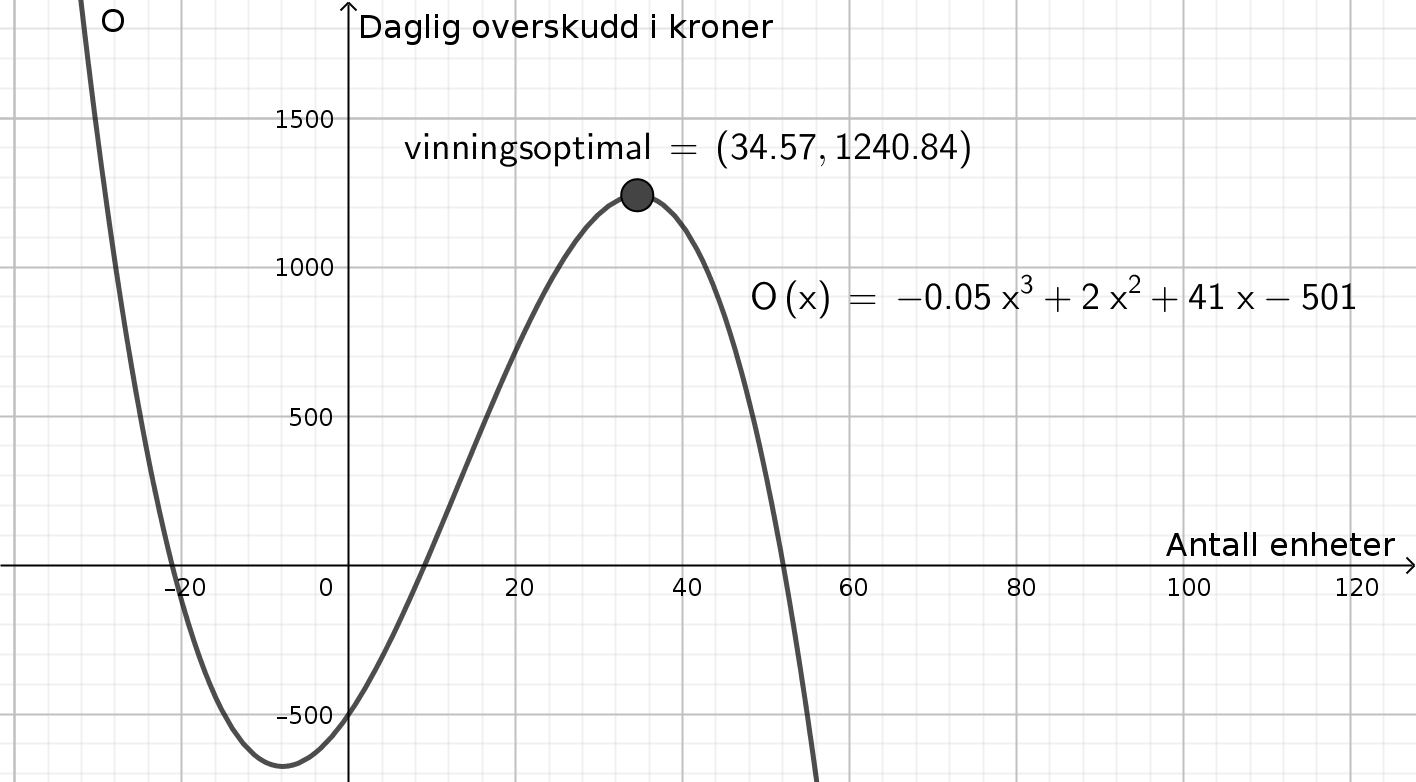
\includegraphics[width=0.7\linewidth]{figs/del2_oppg1bc}
		\caption{Løsning på oppgave 1 a og b, del 2. }
		\label{fig:del2_oppg1bc}
	\end{figure}
	# La inntekten være $I(x) = px$, der $p$ er en ukjent pris.
	Vi må finne minste $O(x) = I(x) - K(x) = px - K(x)$ slik at $O(x)$ er større enn eller lik null, for minst én $x$-verdi.
	Vi får en overskuddsfunksjon som blir
	\begin{align*}
		O(x) &= I(x) - K(x) \\
		&= px -\left[ 0.05x^3 - 2x^2 + px + 501 \right] \\
		&= - 0.05x^3 + 2x^2 + (80 - p)x - 501
	\end{align*}
	Ved å lage en glider for $p$ i Geogebra, ser vi at $O(x) \geq 0$ når $p \leq 79$. Høyeste pris blir \answer{$p = 79$}, og da må bedriften produsere \answer{$x = 27$} varer per dag.
\end{easylist}


\subsection*{Oppgave 2}
\begin{easylist}[enumerate]
	\ListProperties(Style2*=,Numbers=a,Numbers1=l,FinalMark={)})
	# La oss oppsummere oppgaven i en tabell.
	Vi lar $b = 40000$ være det årlige beløpet, og $r = 1.05$ være rentefaktoren.
	La $P_n$ være pengene etter $n$ år, da er $P_n = P_{n-1} r + b$ fordi vi får renter på forrige års sum, og deretter setter vi inn et nytt beløp.
	En tabell som viser 15 år med sparing er vist nedenfor.
	\begin{center}
		\begin{tabular}{lll}
			\textbf{Innskudd} & \textbf{Dato} & \textbf{Penger} \\ \hline
			1 & 1. juli 2018 & $b$ \\
			2 & 1. juli 2019 & $br + b$ \\
			3 & 1. juli 2020 & $br^2 + br + b$ \\
			$\, \vdots$ & $\qquad \vdots$ & $\qquad \vdots$ \\
			15 & 1. juli 2032 & $br^{14} + br^{13} + \dots + br + b$ \\
			 & 1. juli 2033 & $\left(br^{14} + br^{13} + \dots + br + b\right) r$ \\
		\end{tabular}
	\end{center}
	Ett år etter siste innbetaling får Eirik renter på forrige beløp,
	da ender han opp med
	\begin{equation*}
		\left(br^{14} + \dots + br + b\right)r = b\left(\frac{1 - r^{15}}{1 - r}\right)r 
		= 40000\left(\frac{1 - 1.05^{15}}{1 - 1.05}\right)1.05 = \answer{906299.67}
	\end{equation*}
	For å gjøre utregningen i CAS taster vi inn \\
	\verb|Sum(b * r^i, i, 0, 14) * r| \\
	etter å ha definert \verb|b| og \verb|r| i CAS. Vi får samme svar som ovenfor.
	# La $T = 906299.67$ være løsningen på forrige deloppgave, og la $u$ være det ukjente årlige uttaket.
	Da har Eirik $T-u$ kroner 1. juli 2033, $Tr - ur - u$ kroner 1. juli 2034, og så videre. Vi setter opp tabell.
	\begin{center}
		\begin{tabular}{lll}
			\textbf{Uttak} & \textbf{Dato} & \textbf{Penger} \\ \hline
			0 & 1. juli 2033 & $T - u$ \\
			1 & 1. juli 2034 & $Tr - ur - u$ \\
			2 & 1. juli 2035 & $Tr^2 -ur^2 - ur - u$ \\
			$\, \vdots$ & $\qquad \vdots$ & $\qquad \vdots$ \\
			14 & 1. juli 2047 & $Tr^{14} - u \left(r^{14} + \dots + r + 1\right)$  
		\end{tabular}
	\end{center}
	 Den 1. juli 2047 skal han ha $0$ kroner igjen. Vi får da likningen 
	 \begin{equation*}
	 	Tr^{14} - u \left(r^{14} + \dots + r + 1\right) = 0
	 \end{equation*}
	 som vi løser i CAS med \\
	 \verb|NLøs({T * r^14 - u * Sum(r^i, i, 0, 14) = 0}, {u})| \\
	 og får \answer{$83157.13$ kroner} som svar.
	# For at fondet skal kunne betale ut i all fremtid, må utbetalingen og rentene kansellere hverandre.
	Vi ønsker at Eirik har det samme på konto før utbetaling hvert år.
	Den 1. juli 2033 har han $T$ kroner før utbetaling. 
	Så kommer en utbetaling, og han har $T - u$ kroner.
	Neste år får han renter og har $(T-u)r$ kroner før utbetaling.
	Vi ønsker at han skal ha like mye før utbetaling hvert år, da får vi likningen $(T - u)r = T$, som vi kan løse for den ukjente $u$ slik
	\begin{equation*}
		(T - u)r = T \quad \Rightarrow \quad u = \frac{T(r-1)}{r}
		 = \frac{906299.67(1.05-1)}{1.05} = \answer{43157.13}
	\end{equation*}
	# Vi setter uttaket til $u = 30000$ og lar $k = 1.1$ være vekstfaktoren til uttaksbeløpet.
	Eirik tar ut $u$ kroner i 2033, $uk$ i 2034, $uk^2$ i 2035, og så videre.
	Vi setter opp en tabell med penger på kontoen rett etter uttak.
	\begin{center}
	\begin{tabular}{lll}
		\textbf{Uttak} & \textbf{Dato} & \textbf{Penger} \\ \hline
		0 & 1. juli 2033 & $T - u$ \\
		1 & 1. juli 2034 & $(T-u)r - uk = Tr - u(r + k)$ \\
		2 & 1. juli 2035 & $((T-u)r - uk)r - uk^2 = Tr^2 - u(r^2 +rk + k^2)$ \\
		$\, \vdots$ & $\qquad \vdots$ & $\qquad \vdots$ \\
		14 & 1. juli 2047 & $Tr^n - u \sum_{i=0}^{n} r^{n-i} k^i$  
	\end{tabular}
	\end{center}
	Vi løser med følgende Geogebra kommando i CAS \\
	\verb|NLøs({T * r^n - u * Sum(r^(n - i) * k^i, i, 0, n) = 0}, {n})| \\
	og får $n = 18.16$.
	Når $n = 18$ er det omtrent 27.7 tusen kroner på konto etter uttak, mens når $n = 19$ er det $-154.3$ tusen kroner på konto etter uttak.
	Med andre ord går kontoen tom når $n=19$, altså \answer{1. juli 2052}, da tar vi ut 27.7 tusen og tømmer kontoen.
	
	TODO: Vis hvordan man kan bruke nåverdi til å løse denne. 
\end{easylist}

\subsection*{Oppgave 3}
\begin{easylist}[enumerate]
	\ListProperties(Style2*=,Numbers=a,Numbers1=l,FinalMark={)})
	# La $X$ være vekten på en flaske, da er $X$ normalfordelt med $\mu = 250$ og $\sigma = 3$.
	Sannsynligheten for at en flaske veier for lite er $P(X< 245)$.
	Dette regner vi enkelt ut i sannsynlighetskalkulatoren i Geogebra, og får
	\begin{equation*}
		\answer{P(X < 245) = 0.0478 \approx 4.8 \%}
	\end{equation*}
	# La $Y$ være antall flasker som veier for lite,
	da er $Y$ binomisk fordelt med $n = 15$ og $p = 0.0478$.
	Sannsynligheten for at én eller flere flasker veier for lite er $P(Y \geq 1)$, vi kan regne dette ut på følgende måte
	\begin{equation*}
		P(Y \geq 1) = 1 - P(Y = 0) = 1 - \binom{15}{0}p^0(1-p)^{15} = 1 - (1 - p)^{15} = 0.5203 = \answer{52.0\%}
	\end{equation*}
	Det er nok enda enklere å bruke sannsynlighetskalkulatoren. Vi får samme svar uansett, men denne formelen er grei å ha til neste oppgave.
	# Sannsynligheten for at en flaske veier for lite er $P(Y \geq 1) = 1 -  (1-p)^{15}$, vi ønsker å finne $p$ slik at $P(Y \geq 1) < 0.1$, da får vi ulikheten
	\begin{align*}
	1  - (1-p)^{15} & < 0.1 \\
	0.9 & < (1-p)^{15} \\
	p & < 1 - 0.9^{1/15} \approx \answer{0.007}
	\end{align*}
	Vi ser at sannsynligheten for at én flaske veier for lite kan maksimalt være 0.7\% dersom sannsynligheten for at en eske inneholder flasker som veier for lite maksimalt skal være høyst 10\%.
	# Vi må finne $\mu$ slik at $P(X \leq 245) = 0.007$. Vi standardiserer og sammenligner med $z$ slik at $P(Z < z) = 0.007$, enten via tabell eller via sannsynlighetskalkulatoren i Geogebra.
	\begin{align*}
		P(X \leq 245) &= 0.007 \\
		P\left(Z \leq \frac{245 - \mu}{3} \right) &= 0.007 \\
		P\left(Z \leq - 2.457 \right) &= 0.007 
	\end{align*}
	Dette gir oss likningen $(245 - \mu)/3 = - 2.457$, som vi løser for \answer{$\mu = 252.37$}.
	Dette svaret kan vi dobbelsjekke ved å lage en fordeling med $\mu = 252.37$ og $\sigma = 3$ i sannsynlighetskalkulatoren i Geogebra, og verifisere at $P(X < 245) = 0.007$.
\end{easylist}




\end{document}


